\chapter{Results and Discussion} \label{chap:results}

\section{Overall Performance}
\subsection{Trauma Data Set}
Tables \ref{tab:overall-tr-acc} and \ref{tab:overall-tr-auc} show the best
accuracy and AUC results for each of the feature selection methods for each
classifier. The best accuracy was 77.81\%, achieved using the $k$-NN algorithm
with 1 nearest neighbour, a discretised data set, and feature selection using a
C4.5 wrapper. The best AUC of 0.846 was achieved using logistic regression with
features selected by a correlation coefficient threshold of 0.1, and again
using the discretised data set.

\begin{table}[htbp]
\caption{Overall best accuracy of each classifier with a particular feature selection method on the trauma data set. * indicates that results were identical regardless of discretisation. D indicates that discretisation was used, and $t$ is the threshold at which the feature selector was applied. The absence of * or D means that not discretising produced a better result. The best result for each classifier is highlighted in bold, with ties broken in favour of the smallest feature set.}
\label{tab:overall-tr-acc}
\resizebox{\linewidth}{!}{%
\begin{tabular}{|l|cccccccc|}
\hline
Classifier & None & Baseline & Expert & CFS & C4.5 Wrapper & Correlation & IG & 1R \\ \hline
ZeroR & 66.91* & 66.91* & 66.91* & 66.91* & 66.91* & 66.91* & 66.91* & 66.91* \\
1R & 71.95 & 66.91* & \begin{tabular}[c]{@{}c@{}}70.64\\ D\end{tabular} & \textbf{72.01} & 71.93 & \begin{tabular}[c]{@{}c@{}}71.91\\ t=0.01\end{tabular} & \begin{tabular}[c]{@{}c@{}}71.95\\ t=0.001\end{tabular} & \begin{tabular}[c]{@{}c@{}}71.97\\ t=66.905\end{tabular} \\
NB & \begin{tabular}[c]{@{}c@{}}73.83\\ D\end{tabular} & 74.62* & \begin{tabular}[c]{@{}c@{}}73.19\\ D\end{tabular} & \begin{tabular}[c]{@{}c@{}}73.4\\ D\end{tabular} & \textbf{\begin{tabular}[c]{@{}c@{}}75.8\\ D\end{tabular}} & \begin{tabular}[c]{@{}c@{}}74.85\\ D, t=0.125\end{tabular} & \begin{tabular}[c]{@{}c@{}}74.45\\ D, t=0.01\end{tabular} & \begin{tabular}[c]{@{}c@{}}72.37\\ D, t=69.905\end{tabular} \\
DT & \begin{tabular}[c]{@{}c@{}}75\\ D\end{tabular} & 74.38* & \begin{tabular}[c]{@{}c@{}}76.39\\ D\end{tabular} & 75.4 & \textbf{\begin{tabular}[c]{@{}c@{}}77.52\\ D\end{tabular}} & \begin{tabular}[c]{@{}c@{}}76.05\\ D, t=0.11\end{tabular} & \begin{tabular}[c]{@{}c@{}}76.17\\ D, t=0.01\end{tabular} & \begin{tabular}[c]{@{}c@{}}73.49\\ t=66.905\end{tabular} \\
LR & \begin{tabular}[c]{@{}c@{}}77.62\\ D\end{tabular} & 75.06* & \begin{tabular}[c]{@{}c@{}}76.45\\ D\end{tabular} & 74.14 & \begin{tabular}[c]{@{}c@{}}76.3\\ D\end{tabular} & \textbf{\begin{tabular}[c]{@{}c@{}}77.7\\ D, t=0\end{tabular}} & \begin{tabular}[c]{@{}c@{}}77.65\\ D, t=0\end{tabular} & \begin{tabular}[c]{@{}c@{}}74.4\\ D, t=66.905\end{tabular} \\
SVM & \begin{tabular}[c]{@{}c@{}}77.39\\ D\end{tabular} & 74.47* & \begin{tabular}[c]{@{}c@{}}75.67\\ D\end{tabular} & \begin{tabular}[c]{@{}c@{}}72.57\\ D\end{tabular} & \begin{tabular}[c]{@{}c@{}}75.26\\ D\end{tabular} & \begin{tabular}[c]{@{}c@{}}77.42\\ D, t=0.1\end{tabular} & \textbf{\begin{tabular}[c]{@{}c@{}}77.53\\ D, t=0.005\end{tabular}} & \begin{tabular}[c]{@{}c@{}}73.83\\ D, t=66.905\end{tabular} \\
1NN & \begin{tabular}[c]{@{}c@{}}71.22\\ D\end{tabular} & 70.28* & \begin{tabular}[c]{@{}c@{}}72.56\\ D\end{tabular} & 74.44 & \textbf{\begin{tabular}[c]{@{}c@{}}77.81\\ D\end{tabular}} & \begin{tabular}[c]{@{}c@{}}74.75\\ D, t=0.15\end{tabular} & \begin{tabular}[c]{@{}c@{}}73.26\\ D, t=0.01\end{tabular} & \begin{tabular}[c]{@{}c@{}}73.78\\ t=68.905\end{tabular} \\
20NN & \begin{tabular}[c]{@{}c@{}}75.9\\ D\end{tabular} & 73.59* & \begin{tabular}[c]{@{}c@{}}75.51\\ D\end{tabular} & 75.3 & \begin{tabular}[c]{@{}c@{}}76.48\\ D\end{tabular} & \begin{tabular}[c]{@{}c@{}}76.26\\ D, t=0.125\end{tabular} & \textbf{\begin{tabular}[c]{@{}c@{}}76.56\\ D, t=0.005\end{tabular}} & \begin{tabular}[c]{@{}c@{}}73.56\\ t=68.905\end{tabular} \\
RD & \begin{tabular}[c]{@{}c@{}}76.92\\ D\end{tabular} & 69.68* & \begin{tabular}[c]{@{}c@{}}76.19\\ D\end{tabular} & 74.38 & \textbf{\begin{tabular}[c]{@{}c@{}}77.22\\ D\end{tabular}} & \begin{tabular}[c]{@{}c@{}}76.87\\ D, t=0.05\end{tabular} & \begin{tabular}[c]{@{}c@{}}76.82\\ D, t=0.001\end{tabular} & \begin{tabular}[c]{@{}c@{}}73.83\\ D, t=66.905\end{tabular} \\
K* & \begin{tabular}[c]{@{}c@{}}71.4\\ D\end{tabular} & 72.20* & \begin{tabular}[c]{@{}c@{}}75.08\\ D\end{tabular} & 75.58 & \textbf{\begin{tabular}[c]{@{}c@{}}77.27\\ D\end{tabular}} & \begin{tabular}[c]{@{}c@{}}75.07\\ D, t=0.15\end{tabular} & \begin{tabular}[c]{@{}c@{}}74.08\\ D, t=0.01\end{tabular} & \begin{tabular}[c]{@{}c@{}}73.45\\ t=68.905\end{tabular} \\
MLP & \begin{tabular}[c]{@{}c@{}}73.79\\ D\end{tabular} & 73.03* & \begin{tabular}[c]{@{}c@{}}73.45\\ D\end{tabular} & \begin{tabular}[c]{@{}c@{}}73.38\\ D\end{tabular} & \textbf{\begin{tabular}[c]{@{}c@{}}76.66\\ D\end{tabular}} & \begin{tabular}[c]{@{}c@{}}74.65\\ t=0.15\end{tabular} & \begin{tabular}[c]{@{}c@{}}74.03\\ D, t=0.001\end{tabular} & \begin{tabular}[c]{@{}c@{}}71.94\\ D, t=66.905\end{tabular} \\ \hline
\end{tabular}
}
\end{table}



\begin{table}[htbp]
\resizebox{\textwidth}{!}{%
\begin{tabular}{l|cccccccc}
Classifier & None & Baseline & Expert & CFS & C4.5 Wrapper & Correlation & IG & 1R \\ \hline
ZeroR & 0.498* & 0.498* & 0.498* & 0.498* & 0.498* & 0.498* & 0.498* & 0.498* \\
1R & 0.67 & 0.5* & 0.581* & 0.668 & 0.668 & \begin{tabular}[c]{@{}c@{}}0.669\\ t=0.01\end{tabular} & \begin{tabular}[c]{@{}c@{}}0.669\\ t=0.005\end{tabular} & \textbf{\begin{tabular}[c]{@{}c@{}}0.67\\ t=69.905\end{tabular}} \\
NB & \begin{tabular}[c]{@{}c@{}}0.828\\ D\end{tabular} & 0.804* & \begin{tabular}[c]{@{}c@{}}0.806\\ D\end{tabular} & \begin{tabular}[c]{@{}c@{}}0.815\\ D\end{tabular} & \begin{tabular}[c]{@{}c@{}}0.827\\ D\end{tabular} & \begin{tabular}[c]{@{}c@{}}0.829\\ D, t=0.125\end{tabular} & \textbf{\begin{tabular}[c]{@{}c@{}}0.832\\ D, t=0.01\end{tabular}} & \begin{tabular}[c]{@{}c@{}}0.8\\ D, t=66.905\end{tabular} \\
DT & \begin{tabular}[c]{@{}c@{}}0.756\\ D\end{tabular} & 0.772* & \begin{tabular}[c]{@{}c@{}}0.786\\ D\end{tabular} & \begin{tabular}[c]{@{}c@{}}0.793\\ D\end{tabular} & \textbf{\begin{tabular}[c]{@{}c@{}}0.806\\ D\end{tabular}} & \begin{tabular}[c]{@{}c@{}}0.799\\ D, t=0.15\end{tabular} & \begin{tabular}[c]{@{}c@{}}0.787\\ D, t=0.01\end{tabular} & \begin{tabular}[c]{@{}c@{}}0.766\\ D, t=66.905\end{tabular} \\
LR & \begin{tabular}[c]{@{}c@{}}0.844\\ D\end{tabular} & 0.812* & \begin{tabular}[c]{@{}c@{}}0.825\\ D\end{tabular} & \begin{tabular}[c]{@{}c@{}}0.819\\ D\end{tabular} & \begin{tabular}[c]{@{}c@{}}0.831\\ D\end{tabular} & \textbf{\begin{tabular}[c]{@{}c@{}}0.846\\ D, t=0.1\end{tabular}} & \begin{tabular}[c]{@{}c@{}}0.844\\ D, t=0\end{tabular} & \begin{tabular}[c]{@{}c@{}}0.811\\ D, t=66.905\end{tabular} \\
SVM & \begin{tabular}[c]{@{}c@{}}0.843\\ D\end{tabular} & 0.787* & 0.807 & \begin{tabular}[c]{@{}c@{}}0.782\\ D\end{tabular} & 0.806 & \textbf{\begin{tabular}[c]{@{}c@{}}0.844\\ D, t=0.1\end{tabular}} & \begin{tabular}[c]{@{}c@{}}0.842\\ D, t=0\end{tabular} & \begin{tabular}[c]{@{}c@{}}0.724\\ D, t=66.905\end{tabular} \\
1NN & \begin{tabular}[c]{@{}c@{}}0.726\\ D\end{tabular} & 0.719* & \begin{tabular}[c]{@{}c@{}}0.760\\ D\end{tabular} & \begin{tabular}[c]{@{}c@{}}0.798\\ D\end{tabular} & \textbf{\begin{tabular}[c]{@{}c@{}}0.816\\ D\end{tabular}} & \begin{tabular}[c]{@{}c@{}}0.798\\ D, t=0.2\end{tabular} & \begin{tabular}[c]{@{}c@{}}0.768\\ t=0.1\end{tabular} & \begin{tabular}[c]{@{}c@{}}0.778\\ t=68.905\end{tabular} \\
20NN & \begin{tabular}[c]{@{}c@{}}0.827\\ D\end{tabular} & 0.792* & \begin{tabular}[c]{@{}c@{}}0.808\\ D\end{tabular} & 0.814 & \begin{tabular}[c]{@{}c@{}}0.828\\ D\end{tabular} & \begin{tabular}[c]{@{}c@{}}0.831\\ D, t=0.1\end{tabular} & \textbf{\begin{tabular}[c]{@{}c@{}}0.832\\ D, t=0.01\end{tabular}} & \begin{tabular}[c]{@{}c@{}}0.799\\ D, t=66.905\end{tabular} \\
RD & \begin{tabular}[c]{@{}c@{}}0.834\\ D\end{tabular} & 0.742* & \begin{tabular}[c]{@{}c@{}}0.807\\ D\end{tabular} & 0.81 & \begin{tabular}[c]{@{}c@{}}0.825\\ D\end{tabular} & \textbf{\begin{tabular}[c]{@{}c@{}}0.836\\ D, t=0.01\end{tabular}} & \begin{tabular}[c]{@{}c@{}}0.834\\ D, t=0.005\end{tabular} & \begin{tabular}[c]{@{}c@{}}0.791\\ D, t=66.905\end{tabular} \\
K* & \begin{tabular}[c]{@{}c@{}}0.768\\ D\end{tabular} & 0.774* & \begin{tabular}[c]{@{}c@{}}0.803\\ D\end{tabular} & 0.815 & \textbf{\begin{tabular}[c]{@{}c@{}}0.838\\ D\end{tabular}} & \begin{tabular}[c]{@{}c@{}}0.82\\ D, t=0.15\end{tabular} & \begin{tabular}[c]{@{}c@{}}0.802\\ D, t=0.01\end{tabular} & \begin{tabular}[c]{@{}c@{}}0.787\\ t=68.905\end{tabular} \\
MLP & \begin{tabular}[c]{@{}c@{}}0.803\\ D\end{tabular} & 0.781* & \begin{tabular}[c]{@{}c@{}}0.784\\ D\end{tabular} & \begin{tabular}[c]{@{}c@{}}0.802\\ D\end{tabular} & \textbf{\begin{tabular}[c]{@{}c@{}}0.825\\ D\end{tabular}} & \begin{tabular}[c]{@{}c@{}}0.818\\ t=0.15\end{tabular} & \begin{tabular}[c]{@{}c@{}}0.803\\ D, t=0\end{tabular} & \begin{tabular}[c]{@{}c@{}}0.772\\ D, t=68.905\end{tabular} \\
\end{tabular}
}
\caption{Overall best AUC of each classifier with a particular feature selection method on the trauma data set. * indicates that results were identical regardless of discretisation. D indicates that discretisation was used, and $t$ is the threshold at which the feature selector was applied. The absence of * or D means that not discretising produced a better result. The best result for each classifier is highlighted in bold, with ties broken in favour of the smallest feature set.}
\label{tab:overall-tr-auc}
\end{table}


Recall that in order for our work to be comparable to that of previous work on
trauma LOS prediction by Dinh et al. \cite{Dinh2013a}, we use the same data set
that they used, and also tested the features they used as one of the manual
feature selection methods. From Table \ref{tab:overall-tr-acc} we can see that
the best accuracy achieved using their features is 75.06\% with logistic
regression. It is worth noting that our best accuracy, using $k$-NN with 1
nearest neighbour, improves upon the accuracy that they achieved by 2.75\%
while using only 11 features (compared to the 19 they used). These 11 features
make up only 14.1\% of all features in the data set, and performed better than
the 11 features selected manually by the domain expert.

Despite our inclusion of accuracy as an evaluation metric, the AUC is what Dinh
et al. used to evaluate the ability of their logistic regression classifier to
discriminate between the two LOS classes. Using their features, the best AUC
was 0.812 with logistic regression, and our best result was 0.846, also with
logistic regression. However, this was using the discretised data set with 29
features selected by correlation coefficient at a threshold of 0.1.
Although our logistic regression classifier exhibited an AUC improvement of
0.034, it required roughly 50\% more features than the baseline of 19 features.

Although $k$-NN with 1 nearest neighbour had the highest accuracy (77.81\%) out
of all combinations of classifiers and feature selection methods for this data
set, we should mention that logistic regression came a very close second with
77.7\%, outperforming more sophisticated approaches such as SVM and MLP. It
also achieved a higher AUC, and all while being faster to train.

We would also like to highlight the importance of discretisation on improving
performance: in Tables \ref{tab:overall-tr-acc} and
\ref{tab:overall-tr-auc} the majority of the quoted results are from applying
the learning algorithm and feature selection method on the discretised data.
This indicates that discretisation produced a better result than applying the
same classifier and feature selector on the non-discretised data.

\subsection{General Data Set}
For the general hospital data set, we report the best accuracy and AUC results
for each combination of classifier and feature selection method in Tables
\ref{tab:overall-pt-acc} and \ref{tab:overall-pt-auc}. The most accurate
classifier was the C4.5 decision tree using all 14 features.
This result was the same
regardless of whether or not discretisation was first applied to the data set.
The best AUC result was achieved by three classifiers: logistic regression, SVM
and K*, with an AUC of 0.994. Logistic regression and K* achieved this AUC with
an information gain feature selector with threshold 0.05, and SVM with a
correlation coefficient selector at a 0.1 threshold. We consider logistic
regression and K* to be superior to the SVM in this case because they achieved
the same AUC with only 8 features, whereas the SVM required 10.

\begin{table}[htbp]
\label{tab:overall-pt-acc}
\caption{Overall best accuracy of each classifier with a particular feature selection method on the general hospital data set. * indicates that results were identical regardless of discretisation. D indicates that discretisation was used, and $t$ is the threshold at which the feature selector was applied. The absence of * or D means that not discretising produced a better result. The best result for each classifier is highlighted in bold, with ties broken in favour of the smallest feature set.}
\begin{tabular}{|l|cccccc|}
\hline
Classifier & None & CFS & C4.5 Wrapper & Correlation & IG & 1R \\ \hline
ZeroR & 75.64* & 75.64* & 75.64* & 75.64* & 75.64* & 75.64* \\
1R & 92.88* & 92.88* & 92.88* & 92.88* & 92.88* & 92.88* \\
NB & 93.66* & 93.06* & 93* & \textbf{\begin{tabular}[c]{@{}c@{}}93.72*\\ t=0.125\end{tabular}} & \begin{tabular}[c]{@{}c@{}}93.66*\\ t=0\end{tabular} & \begin{tabular}[c]{@{}c@{}}93.66*\\ t=74.405\end{tabular} \\
DT & \textbf{98.23*} & 96.45* & 97.43* & \begin{tabular}[c]{@{}c@{}}98.23\\ t=0\end{tabular} & \begin{tabular}[c]{@{}c@{}}98.23\\ t=0.001\end{tabular} & \begin{tabular}[c]{@{}c@{}}98.23\\ t=74.405\end{tabular} \\
LR & \textbf{97.93*} & 96.46* & 97.19* & \begin{tabular}[c]{@{}c@{}}97.93\\ t=0.01\end{tabular} & \begin{tabular}[c]{@{}c@{}}97.93\\ t=0.001\end{tabular} & \begin{tabular}[c]{@{}c@{}}97.93\\ t=74.405\end{tabular} \\
SVM & \textbf{98.01*} & 96.46* & 97.14* & \begin{tabular}[c]{@{}c@{}}98.01\\ t=0.01\end{tabular} & \begin{tabular}[c]{@{}c@{}}98.01\\ t=0.001\end{tabular} & \begin{tabular}[c]{@{}c@{}}98.01\\ t=74.405\end{tabular} \\
1NN & \begin{tabular}[c]{@{}c@{}}96.93\\ D\end{tabular} & 96.45* & 97.36* & \textbf{\begin{tabular}[c]{@{}c@{}}97.59*\\ t=0.15\end{tabular}} & \begin{tabular}[c]{@{}c@{}}97.57*\\ t=0.1\end{tabular} & \begin{tabular}[c]{@{}c@{}}97.43*\\ t=76.905\end{tabular} \\
20NN & 96.85 & 96.24* & 97.15* & \textbf{\begin{tabular}[c]{@{}c@{}}97.3\\ T=0.15\end{tabular}} & \begin{tabular}[c]{@{}c@{}}97.15\\ T=0.1\end{tabular} & \begin{tabular}[c]{@{}c@{}}96.86\\ T=68.905\end{tabular} \\
RD & 97.34 & 79.1* & 95.45* & \begin{tabular}[c]{@{}c@{}}97.3\\ t=0\end{tabular} & \textbf{\begin{tabular}[c]{@{}c@{}}97.36\\ t=0\end{tabular}} & \begin{tabular}[c]{@{}c@{}}97.34\\ t=68.905\end{tabular} \\
K* & 97.36 & 92.94* & 96.53* & \textbf{\begin{tabular}[c]{@{}c@{}}97.46*\\ t=0.05\end{tabular}} & \begin{tabular}[c]{@{}c@{}}97.46*\\ t=0.01\end{tabular} & \begin{tabular}[c]{@{}c@{}}97.36\\ t=74.405\end{tabular} \\
MLP & 98.16 & 96.45* & 97.35* & \textbf{\begin{tabular}[c]{@{}c@{}}98.22*\\ t=0.05\end{tabular}} & \begin{tabular}[c]{@{}c@{}}98.22*\\ t=0.01\end{tabular} & \begin{tabular}[c]{@{}c@{}}98.16\\ t=74.405\end{tabular} \\ \hline
\end{tabular}
\end{table}

\begin{table}[htbp]
\caption{Overall best AUC of each classifier with a particular feature selection method on the general hospital data set. * indicates that results were identical regardless of discretisation. D indicates that discretisation was used, and $t$ is the threshold at which the feature selector was applied. The absence of * or D means that not discretising produced a better result. The best result for each classifier is highlighted in bold, with ties broken in favour of the smallest feature set.}
\label{tab:overall-pt-auc}
\begin{tabular}{|l|cccccc|}
\hline
Classifier & None & CFS & C4.5 Wrapper & Correlation & IG & 1R \\ \hline
ZeroR & 0.5* & 0.5* & 0.5* & 0.5* & 0.5* & 0.5* \\
1R & 0.858* & 0.858* & 0.858* & 0.858* & 0.858* & 0.858* \\
NB & \begin{tabular}[c]{@{}c@{}}0.979\\ D\end{tabular} & 0.982* & \textbf{0.983*} & \begin{tabular}[c]{@{}c@{}}0.981*\\ t=0.15\end{tabular} & \begin{tabular}[c]{@{}c@{}}0.979*\\ t=0.01\end{tabular} & \begin{tabular}[c]{@{}c@{}}0.979*\\ t=74.405\end{tabular} \\
DT & \textbf{0.989} & 0.981* & 0.984* & \begin{tabular}[c]{@{}c@{}}0.989\\ t=0.01\end{tabular} & \begin{tabular}[c]{@{}c@{}}0.989*\\ t=0.001\end{tabular} & \begin{tabular}[c]{@{}c@{}}0.989*\\ t=74.405\end{tabular} \\
LR & 0.994* & 0.981* & 0.990* & \begin{tabular}[c]{@{}c@{}}0.994*\\ t=0.1\end{tabular} & \textbf{\begin{tabular}[c]{@{}c@{}}0.994*\\ t=0.05\end{tabular}} & \begin{tabular}[c]{@{}c@{}}0.994*\\ t=74.405\end{tabular} \\
SVM & 0.994* & 0.971* & 0.981* & \textbf{\begin{tabular}[c]{@{}c@{}}0.994*\\ t=0.1\end{tabular}} & \begin{tabular}[c]{@{}c@{}}0.994*\\ t=0.01\end{tabular} & \begin{tabular}[c]{@{}c@{}}0.994*\\ t=74.405\end{tabular} \\
1NN & \begin{tabular}[c]{@{}c@{}}0.979\\ D\end{tabular} & 0.982* & \textbf{0.991*} & \begin{tabular}[c]{@{}c@{}}0.991*\\ t=0.15\end{tabular} & \begin{tabular}[c]{@{}c@{}}0.990*\\ t=0.1\end{tabular} & \begin{tabular}[c]{@{}c@{}}0.989*\\ t=76.905\end{tabular} \\
20NN & 0.992* & 0.981* & 0.991* & \textbf{\begin{tabular}[c]{@{}c@{}}0.992*\\ t=0.15\end{tabular}} & \begin{tabular}[c]{@{}c@{}}0.992*\\ t=0.05\end{tabular} & \begin{tabular}[c]{@{}c@{}}0.992*\\ t=74.405\end{tabular} \\
RD & 0.993* & 0.794* & 0.986* & \textbf{\begin{tabular}[c]{@{}c@{}}0.993*\\ t=0.05\end{tabular}} & \begin{tabular}[c]{@{}c@{}}0.993*\\ t=0.005\end{tabular} & \begin{tabular}[c]{@{}c@{}}0.993*\\ t=74.405\end{tabular} \\
K* & 0.994 & 0.980* & 0.989* & \begin{tabular}[c]{@{}c@{}}0.994*\\ t=0.1\end{tabular} & \textbf{\begin{tabular}[c]{@{}c@{}}0.994*\\ t=0.05\end{tabular}} & \begin{tabular}[c]{@{}c@{}}0.994\\ t=74.405\end{tabular} \\
MLP & 0.990* & 0.983* & 0.992* & \textbf{\begin{tabular}[c]{@{}c@{}}0.993*\\ t=0.15\end{tabular}} & \begin{tabular}[c]{@{}c@{}}0.991*\\ t=0.1\end{tabular} & \begin{tabular}[c]{@{}c@{}}0.990*\\ t=76.905\end{tabular} \\ \hline
\end{tabular}
\end{table}


Due to the general nature of this data set, and because we have defined a
classification problem rather than a regression one, it is difficult to find a
valid baseline for comparison. However, we can still make some remarks about
how this data set performed differently with the same methods that were used
for the trauma LOS data, which will give us valuable insight into the
suitability of classifiers and learning algorithms for predicting the LOS for
various medical domains. In addition, in the following sections it will be
valuable to discuss and compare the important predictive features in this
general data set with features that other researchers have found to be
useful in predicting length of hospital stay.

We note that, unlike for the trauma data set, discretisation does not improve
the accuracy or the AUC of almost all of the classifier and feature selection
combinations. This is likely due to the presence of only one numeric feature
(\texttt{prev\_adm}) which, when discretised, was transformed into a nominal
feature with only one value. Classifiers using the discretised
\texttt{prev\_adm} were likely to perform worse because the single value does
not help predict the class (since it will be the same value for both classes)
and is simply noise. Classifiers which used a reduced set of features that
excluded \texttt{prev\_adm} would have the same performance regardless of
discretisation because all other features were nominal and would not have been
affected by discretisation.

\section{Comparison of Feature Selection Methods}
\subsection{Trauma Data Set}
Tables \ref{tab:features-tr-acc} and \ref{tab:features-tr-auc} show the
best accuracy and AUC achieved with each classifier and feature method, with
both discretised and non-discretised results. We did not include the results of
Zero-R as they do not vary with discretisation or feature selection.
The classifier that achieved the
highest accuracy and AUC over most of the feature selection methods was
logistic regression, with accuracies ranging from 74.4\% with 1R feature
selection to 77.7\% with correlation coefficient feature selection. The AUC
performance of logistic regression ranged from 0.811 to 0.846, again with
1R and correlation feature selection respectively.
\begin{table}[htbp]
\caption{Comparison of accuracy (\%) between all feature selection methods for each classifier with and without discretisation, on the trauma data set. The best accuracy for each feature selection method is highlighted in bold, and the best accuracy for each classifier is italicised.}
\label{tab:features-tr-acc}
\resizebox{!}{11cm}{%
\begin{tabular}{|l|cccccccc|}
\hline
 & \multicolumn{1}{l}{None} & Baseline & Expert & CFS & C4.5 Wrapper & Correlation & IG & 1R \\ \hline
\textit{1R} &  &  &  &  &  &  &  &  \\
Discretised & 69.74 & 66.91 & \textit{70.64} & 69.63 & 70.64 & \textit{\begin{tabular}[c]{@{}c@{}}70.64\\ t=0.15\end{tabular}} & \begin{tabular}[c]{@{}c@{}}69.9\\ t=0.01\end{tabular} & \begin{tabular}[c]{@{}c@{}}69.77\\ t=67.905\end{tabular} \\
Not discretised & 71.95 & 66.91 & 70.61 & \textit{72.01} & 71.93 & \begin{tabular}[c]{@{}c@{}}71.91\\ t=0.01\end{tabular} & \begin{tabular}[c]{@{}c@{}}71.95\\ t=0.001\end{tabular} & \begin{tabular}[c]{@{}c@{}}71.97\\ t=66.905\end{tabular} \\
\textit{NB} &  &  &  &  &  &  &  &  \\
Discretised & 73.83 & 74.62 & 73.19 & 73.4 & \textit{75.8} & \begin{tabular}[c]{@{}c@{}}74.85\\ t=0.125\end{tabular} & \begin{tabular}[c]{@{}c@{}}74.45\\ t=0.01\end{tabular} & \begin{tabular}[c]{@{}c@{}}72.37\\ t=69.905\end{tabular} \\
Not discretised & 67.25 & \textit{74.62} & 68.31 & 64.77 & 62.66 & \begin{tabular}[c]{@{}c@{}}71.91\\ t=0.01\end{tabular} & \begin{tabular}[c]{@{}c@{}}67.65\\ t=0.01\end{tabular} & \begin{tabular}[c]{@{}c@{}}66.91\\ t=71.905\end{tabular} \\
\textit{DT} &  &  &  &  &  &  &  &  \\
Discretised & 75 & 74.38 & 76.39 & 74.12 & \textit{77.52} & \begin{tabular}[c]{@{}c@{}}76.05\\ t=0.125\end{tabular} & \begin{tabular}[c]{@{}c@{}}76.17\\ t=0.01\end{tabular} & \begin{tabular}[c]{@{}c@{}}72.71\\ t=69.905\end{tabular} \\
Not discretised & 74.58 & 74.38 & 76.04 & 75.4 & 75.79 & \textit{\begin{tabular}[c]{@{}c@{}}75.93\\ t=0.15\end{tabular}} & \begin{tabular}[c]{@{}c@{}}75.74\\ t=0.01\end{tabular} & \begin{tabular}[c]{@{}c@{}}73.49\\ t=66.905\end{tabular} \\
\textit{LR} &  &  &  &  &  &  &  &  \\
Discretised & \textbf{77.62} & \textbf{75.06} & \textbf{76.45} & 73.99 & 76.3 & \textit{\textbf{\begin{tabular}[c]{@{}c@{}}77.7\\ t=0\end{tabular}}} & \textbf{\begin{tabular}[c]{@{}c@{}}77.65\\ t=0\end{tabular}} & \textbf{\begin{tabular}[c]{@{}c@{}}74.4\\ t=66.905\end{tabular}} \\
Not discretised & 77.1 & \textbf{75.06} & 74.53 & 74.14 & 73.66 & \begin{tabular}[c]{@{}c@{}}77.09\\ t=0.01\end{tabular} & \textit{\begin{tabular}[c]{@{}c@{}}77.13\\ t=0\end{tabular}} & \begin{tabular}[c]{@{}c@{}}73.57\\ t=66.905\end{tabular} \\
\textit{SVM} &  &  &  &  &  &  &  &  \\
Discretised & 77.39 & 74.47 & 75.67 & 72.57 & 75.26 & \begin{tabular}[c]{@{}c@{}}77.42\\ t=0.05\end{tabular} & \textit{\begin{tabular}[c]{@{}c@{}}77.53\\ t=0.005\end{tabular}} & \begin{tabular}[c]{@{}c@{}}73.83\\ t=66.905\end{tabular} \\
Not discretised & 76.72 & 74.47 & 74.48 & 70.59 & 73.58 & \begin{tabular}[c]{@{}c@{}}76.8\\ t=0.01\end{tabular} & \textit{\begin{tabular}[c]{@{}c@{}}76.83\\ t=0\end{tabular}} & \begin{tabular}[c]{@{}c@{}}72.27\\ t=66.905\end{tabular} \\
\textit{1NN} &  &  &  &  &  &  &  &  \\
Discretised & 71.22 & 70.28 & 72.56 & 73.84 & \textit{\textbf{77.81}} & \begin{tabular}[c]{@{}c@{}}74.75\\ t=0.15\end{tabular} & \begin{tabular}[c]{@{}c@{}}73.26\\ t=0.01\end{tabular} & \begin{tabular}[c]{@{}c@{}}72.72\\ t=69.905\end{tabular} \\
Not discretised & 67.4 & 70.28 & 68.77 & 74.44 & \textit{74.94} & \begin{tabular}[c]{@{}c@{}}72.94\\ t=0.2\end{tabular} & \begin{tabular}[c]{@{}c@{}}71.44\\ t=0.1\end{tabular} & \begin{tabular}[c]{@{}c@{}}73.78\\ t=68.905\end{tabular} \\
\textit{20NN} &  &  &  &  &  &  &  &  \\
Discretised & 75.9 & 73.59 & 75.51 & 73.76 & 76.48 & \begin{tabular}[c]{@{}c@{}}76.26\\ t=0.125\end{tabular} & \textit{\begin{tabular}[c]{@{}c@{}}76.56\\ t=0.005\end{tabular}} & \begin{tabular}[c]{@{}c@{}}73.52\\ t=66.905\end{tabular} \\
Not discretised & 73.48 & 73.59 & 72.11 & \textit{75.3} & 74.59 & \begin{tabular}[c]{@{}c@{}}74.99\\ t=0.2\end{tabular} & \begin{tabular}[c]{@{}c@{}}74.42\\ t=0.01\end{tabular} & \begin{tabular}[c]{@{}c@{}}73.56\\ t=68.905\end{tabular} \\
\textit{RD} &  &  &  &  &  &  &  &  \\
Discretised & 76.92 & 69.68 & 76.19 & 73.39 & \textit{77.22} & \begin{tabular}[c]{@{}c@{}}76.87\\ t=0.05\end{tabular} & \begin{tabular}[c]{@{}c@{}}76.82\\ t=0.001\end{tabular} & \begin{tabular}[c]{@{}c@{}}73.82\\ t=66.905\end{tabular} \\
Not discretised & 74.97 & 69.68 & 74.58 & 74.38 & 75.35 & \begin{tabular}[c]{@{}c@{}}76.05\\ t=0.1\end{tabular} & \textit{\begin{tabular}[c]{@{}c@{}}76.16\\ t=0.01\end{tabular}} & \begin{tabular}[c]{@{}c@{}}73.71\\ t=68.905\end{tabular} \\
\textit{K*} &  &  &  &  &  &  &  &  \\
Discretised & 71.4 & 72.2 & 75.08 & 74.43 & \textit{77.27} & \begin{tabular}[c]{@{}c@{}}75.07\\ t=0.15\end{tabular} & \begin{tabular}[c]{@{}c@{}}74.08\\ t=0.01\end{tabular} & \begin{tabular}[c]{@{}c@{}}72.61\\ t=67.905\end{tabular} \\
Not discretised & 67.34 & 72.2 & 72.6 & \textit{\textbf{75.58}} & 75.48 & \begin{tabular}[c]{@{}c@{}}74.77\\ t=0.2\end{tabular} & \begin{tabular}[c]{@{}c@{}}71.15\\ t=0.05\end{tabular} & \begin{tabular}[c]{@{}c@{}}73.45\\ t=68.905\end{tabular} \\
\textit{MLP} &  &  &  &  &  &  &  &  \\
Discretised & 73.79 & 73.03 & 73.45 & 73.38 & \textit{76.66} & \begin{tabular}[c]{@{}c@{}}74.41\\ t=0.15\end{tabular} & \begin{tabular}[c]{@{}c@{}}74.03\\ t=0.001\end{tabular} & \begin{tabular}[c]{@{}c@{}}71.94\\ t=66.905\end{tabular} \\
Not discretised & 71.87 & 73.03 & 72.31 & 73.04 & 73.35 & \textit{\begin{tabular}[c]{@{}c@{}}74.65\\ t=0.15\end{tabular}} & \begin{tabular}[c]{@{}c@{}}72.63\\ t=0.01\end{tabular} & \begin{tabular}[c]{@{}c@{}}70.99\\ t=66.905\end{tabular} \\ \hline
 \end{tabular}
}
\end{table}

\begin{table}[htbp]
\resizebox{!}{11cm}{%
\begin{tabular}{l|cccccccc}
 & None & Baseline & Expert & CFS & C4.5 Wrapper & Correlation & IG & 1R \\ \hline
\textit{1R} &  &  &  &  &  &  &  &  \\
Discretised & 0.569 & 0.5 & 0.581 & 0.569 & 0.581 & \begin{tabular}[c]{@{}c@{}}0.572\\ t=0.1\end{tabular} & \textit{\begin{tabular}[c]{@{}c@{}}0.581\\ t=0.15\end{tabular}} & \begin{tabular}[c]{@{}c@{}}0.571\\ t=68.905\end{tabular} \\
Not discretised & 0.67 & 0.5 & 0.581 & 0.668 & 0.668 & \begin{tabular}[c]{@{}c@{}}0.669\\ t=0.05\end{tabular} & \begin{tabular}[c]{@{}c@{}}0.669\\ t=0.005\end{tabular} & \textit{\begin{tabular}[c]{@{}c@{}}0.67\\ t=69.905\end{tabular}} \\
\textit{NB} &  &  &  &  &  &  &  &  \\
Discretised & 0.828 & 0.804 & 0.806 & 0.815 & 0.827 & \begin{tabular}[c]{@{}c@{}}0.829\\ t=0.125\end{tabular} & \textit{\begin{tabular}[c]{@{}c@{}}0.832\\ t=0.01\end{tabular}} & \begin{tabular}[c]{@{}c@{}}0.8\\ t=66.905\end{tabular} \\
Not discretised & 0.812 & 0.804 & 0.793 & 0.801 & 0.786 & \begin{tabular}[c]{@{}c@{}}0.815\\ t=0.15\end{tabular} & \textit{\begin{tabular}[c]{@{}c@{}}0.817\\ t=0.01\end{tabular}} & \begin{tabular}[c]{@{}c@{}}0.784\\ t=66.905\end{tabular} \\
\textit{DT} &  &  &  &  &  &  &  &  \\
Discretised & 0.756 & 0.772 & 0.786 & 0.793 & \textit{0.806} & \begin{tabular}[c]{@{}c@{}}0.799\\ t=0.15\end{tabular} & \begin{tabular}[c]{@{}c@{}}0.787\\ t=0.01\end{tabular} & \begin{tabular}[c]{@{}c@{}}0.766\\ t=66.905\end{tabular} \\
Not discretised & 0.727 & 0.772 & 0.762 & 0.782 & 0.784 & \textit{\begin{tabular}[c]{@{}c@{}}0.783\\ t=0.2\end{tabular}} & \begin{tabular}[c]{@{}c@{}}0.757\\ t=0.05\end{tabular} & \begin{tabular}[c]{@{}c@{}}0.756\\ t=69.905\end{tabular} \\
\textit{LR} &  &  &  &  &  &  &  &  \\
Discretised & \textbf{0.844} & \textbf{0.812} & \textbf{0.825} & \textbf{0.819} & 0.831 & \textit{\textbf{\begin{tabular}[c]{@{}c@{}}0.846\\ t=0.1\end{tabular}}} & \textbf{\begin{tabular}[c]{@{}c@{}}0.844\\ t=0\end{tabular}} & \textbf{\begin{tabular}[c]{@{}c@{}}0.811\\ t=66.905\end{tabular}} \\
Not discretised & \textit{0.837} & \textbf{0.812} & 0.812 & 0.812 & 0.809 & \textit{\begin{tabular}[c]{@{}c@{}}0.837\\ t=0\end{tabular}} & \textit{\begin{tabular}[c]{@{}c@{}}0.837\\ t=0\end{tabular}} & \begin{tabular}[c]{@{}c@{}}0.798\\ t=66.905\end{tabular} \\
\textit{SVM} &  &  &  &  &  &  &  &  \\
Discretised & 0.843 & 0.787 & 0.767 & 0.782 & 0.796 & \textit{\begin{tabular}[c]{@{}c@{}}0.844\\ t=0.1\end{tabular}} & \begin{tabular}[c]{@{}c@{}}0.842\\ t=0\end{tabular} & \begin{tabular}[c]{@{}c@{}}0.724\\ t=66.905\end{tabular} \\
Not discretised & \textit{0.836} & 0.787 & 0.807 & 0.778 & 0.806 & \textit{\begin{tabular}[c]{@{}c@{}}0.836\\ t=0\end{tabular}} & \textit{\begin{tabular}[c]{@{}c@{}}0.836\\ t=0\end{tabular}} & \begin{tabular}[c]{@{}c@{}}0.704\\ t=66.905\end{tabular} \\
\textit{1NN} &  &  &  &  &  &  &  &  \\
Discretised & 0.726 & 0.719 & 0.76 & 0.798 & \textit{0.816} & \begin{tabular}[c]{@{}c@{}}0.798\\ t=0.2\end{tabular} & \begin{tabular}[c]{@{}c@{}}0.763\\ t=0.05\end{tabular} & \begin{tabular}[c]{@{}c@{}}0.771\\ t=68.905\end{tabular} \\
Not discretised & 0.651 & 0.719 & 0.653 & 0.772 & 0.756 & \begin{tabular}[c]{@{}c@{}}0.752\\ t=0.3\end{tabular} & \begin{tabular}[c]{@{}c@{}}0.768\\ t=0.1\end{tabular} & \textit{\begin{tabular}[c]{@{}c@{}}0.778\\ t=68.905\end{tabular}} \\
\textit{20NN} &  &  &  &  &  &  &  &  \\
Discretised & 0.827 & 0.792 & 0.808 & 0.811 & 0.828 & \begin{tabular}[c]{@{}c@{}}0.831\\ t=0.1\end{tabular} & \textit{\begin{tabular}[c]{@{}c@{}}0.832\\ t=0.01\end{tabular}} & \begin{tabular}[c]{@{}c@{}}0.799\\ t=66.905\end{tabular} \\
Not discretised & 0.799 & 0.792 & 0.77 & \textit{0.814} & 0.803 & \begin{tabular}[c]{@{}c@{}}0.812\\ t=0.2\end{tabular} & \begin{tabular}[c]{@{}c@{}}0.81\\ t=0.01\end{tabular} & \begin{tabular}[c]{@{}c@{}}0.787\\ t=68.905\end{tabular} \\
\textit{RD} &  &  &  &  &  &  &  &  \\
Discretised & 0.834 & 0.742 & 0.807 & 0.806 & 0.825 & \textit{\begin{tabular}[c]{@{}c@{}}0.836\\ t=0.01\end{tabular}} & \begin{tabular}[c]{@{}c@{}}0.834\\ t=0.005\end{tabular} & \begin{tabular}[c]{@{}c@{}}0.791\\ t=66.905\end{tabular} \\
Not discretised & 0.826 & 0.742 & 0.805 & 0.81 & 0.811 & \begin{tabular}[c]{@{}c@{}}0.83\\ t=0.1\end{tabular} & \textit{\begin{tabular}[c]{@{}c@{}}0.831\\ t=0.01\end{tabular}} & \begin{tabular}[c]{@{}c@{}}0.788\\ t=68.905\end{tabular} \\
\textit{K*} &  &  &  &  &  &  &  &  \\
Discretised & 0.768 & 0.774 & 0.803 & 0.813 & \textit{\textbf{0.838}} & \begin{tabular}[c]{@{}c@{}}0.82\\ t=0.15\end{tabular} & \begin{tabular}[c]{@{}c@{}}0.802\\ t=0.01\end{tabular} & \begin{tabular}[c]{@{}c@{}}0.782\\ t=67.905\end{tabular} \\
Not discretised & 0.732 & 0.774 & 0.784 & \textit{0.815} & 0.809 & \begin{tabular}[c]{@{}c@{}}0.811\\ t=0.2\end{tabular} & \begin{tabular}[c]{@{}c@{}}0.779\\ t=0.05\end{tabular} & \begin{tabular}[c]{@{}c@{}}0.787\\ t=68.905\end{tabular} \\
\textit{MLP} &  &  &  &  &  &  &  &  \\
Discretised & 0.803 & 0.781 & 0.784 & 0.802 & \textit{0.825} & \begin{tabular}[c]{@{}c@{}}0.807\\ t=0.15\end{tabular} & \begin{tabular}[c]{@{}c@{}}0.803\\ t=0\end{tabular} & \begin{tabular}[c]{@{}c@{}}0.772\\ t=68.905\end{tabular} \\
Not discretised & 0.78 & 0.781 & 0.774 & 0.799 & 0.804 & \textit{\begin{tabular}[c]{@{}c@{}}0.818\\ t=0.15\end{tabular}} & \begin{tabular}[c]{@{}c@{}}0.788\\ t=0.01\end{tabular} & \begin{tabular}[c]{@{}c@{}}0.752\\ t=68.905\end{tabular} \\
\end{tabular}
}
\caption{Comparison of AUC between all feature selection methods for each classifier with and without discretisation, on the trauma data set. The best AUC for each feature selection method is highlighted in bold, and the best AUC for each classifier is italicised.}
\label{tab:features-tr-auc}
\end{table}


As indicated by italics in the tables, the best accuracy and AUC results for
each classifier resulted from a reduced feature set obtained through a
particular feature selection method. There was at least one feature selector
for each classifier that managed to outperform the same classifier with
no feature selection. This is likely due to the large number of features in
the original data -- after cleaning and preliminary removal of redundant
features, we were still left with over 50. Many of these would still likely
be irrelevant to predicting the class.
Out of 20 combinations of classifiers
and discretisation (the 10 classifiers with and 10 without
discretisation), the C4.5 wrapper method resulted in the best
accuracy for 7 of these combinations, followed by 5 using information gain
and 4 using the correlation coefficient and very few for the other methods.
Under no combination was 1R the best feature selection method to use, as other
methods produced better accuracy.

Focussing our attention on the AUC tells a slightly different story. Here we
find that the correlation coefficient and the information gain are the feature
selectors that give the best AUC for most of the classifiers, and perform
equally well when used in conjunction with logistic regression and SVMs.
Interestingly, although the C4.5
wrapper method selects features which allow classifiers to achieve good
accuracy, only in 2 out of the 20 combinations of classifiers did it give the
best AUC result out of all the feature selectors. 

Note that regardless of whether we consider accuracy or AUC to be more
important in evaluating how our classifiers performed, neither the baseline
feature set from Dinh et al. \cite{Dinh2013a} nor the features suggested by
the domain expert (both of which were manually selected) yielded better
results than automatic feature selection in all but two cases. We did find
that expert selection produced the best accuracy result for 1R (equal with
correlation coefficient selection, but used less features) and that the
baseline feature set produced the best accuracy for Na\"{i}ve Bayes. Neither
feature selection method produced the best AUC result for any classifier.
This is a surprising result because intuitively and in the literature it
has been stated that in a highly specialised field such as medicine, the domain
experts would be best-equipped to make judgements about which features to
use \cite{Witten2005}, and these should give reasonable results. However,
our results show that in attempting to classify patients according to their
LOS, we should consider both manual and automatic approaches.

Recall that $k$-NN with 1 nearest neighbour and C4.5 wrapper feature
selection produced the best accuracy (77.81\%) for the trauma data set, and
logistic regression with correlation coefficient feature selection at a
threshold of 0.1 gave the best AUC (0.846). These two feature selection
methods selected 11 and 29 features respectively, and the features that
were chosen in common between them were: \texttt{operation}, \texttt{bp},
\texttt{iss}, \texttt{lowerlimbnopelvis}, \texttt{age}, \texttt{lowerlimbany}
and \texttt{icu}. This adds evidence to the work of Dinh et al. who found
that \texttt{iss}, \texttt{age} and \texttt{operation} were important
distinguishers of LOS $\leq$ or $>$ 2 days \cite{Dinh2013a}. We also
confirm the findings of Gabbe et al. who found that \texttt{age},
\texttt{iss} and \texttt{bp} were useful in predicting the length of
hospital stay of blunt trauma patients \cite{Gabbe2005}.

Although we were able to achieve higher accuracy and AUC than the baseline,
our best approaches also have a number of limitations which need to be pointed
out. The first point to note is that using a wrapper method of feature
selection is slower than using a filter approach (or manually picking the
features before training), as the learning algorithm used as the wrapper
needs to be invoked at each of the folds of cross-validation. Additionally,
the $k$-NN algorithm becomes slower as the data set increases in the number
of examples. We did not face such a problem during our work, but this will
have to be addressed for larger data sets. It is also common to use more
than one nearest neighbour, so care needs to be taken to find a suitable number
of neighbours for a given problem. Finally, we achieved an improvement
in AUC of 0.034 but this was with 29 features, which is still a fairly large
number. The importance of using a fewer number of features is twofold: not
only does this speed up the training time, it also means that we are able to
make predictions without requiring a lot of information about a patient,
which is a crucial consideration if this is to be implemented for use by
physicians.

\subsection{General Data Set}
Tables \ref{tab:features-pt-acc} and \ref{tab:features-pt-auc} compare the
best accuracy and AUC of each classifier between all the feature selectors
used on the general hospital data set. Again, Zero-R is not included as it
does not vary with discretisation or feature selection. For accuracy, the
best classifier across all feature selectors except CFS was C4.5, and even
then it
was only 0.01\% less accurate than logistic regression and the SVM. Both
logistic regression and SVM achieved 0.994 AUC using no feature selection
as well as correlation, information gain and 1R at the same thresholds. Whereas
in the trauma data set, the MLP did not perform so well compared to many of the
methods, here it produced the best AUC with CFS and C4.5 wrapper feature
selection, resulting in 0.983 and 0.992 AUC respectively.
\begin{table}[htbp]
\resizebox{!}{11cm}{%
\begin{tabular}{l|cccccc}
 & None & CFS & C4.5 Wrapper & Correlation & IG & 1R \\
\hline
 \textit{1R} &  &  &  &  &  &  \\
 Discretised & 92.88 & 92.88 & 92.88 & 92.88 & 92.88 & 92.88 \\
 Not discretised & 92.88 & 92.88 & 92.88 & 92.88 & 92.88 & 92.88 \\
 \textit{NB} &  &  &  &  &  &  \\
 Discretised & 93.66 & 93.06 & 93 & \textit{\begin{tabular}[c]{@{}c@{}}93.72\\ t=0.125\end{tabular}} & \begin{tabular}[c]{@{}c@{}}93.66\\ t=0\end{tabular} & \begin{tabular}[c]{@{}c@{}}93.66\\ t=74.405\end{tabular} \\
 Not discretised & 93.66 & 93.06 & 93 & \textit{\begin{tabular}[c]{@{}c@{}}93.72\\ t=0.125\end{tabular}} & \begin{tabular}[c]{@{}c@{}}93.66\\ t=0\end{tabular} & \begin{tabular}[c]{@{}c@{}}93.66\\ t=74.405\end{tabular} \\
 \textit{DT} &  &  &  &  &  &  \\
 Discretised & \textit{\textbf{98.23}} & 96.45 & \textbf{97.43} & \begin{tabular}[c]{@{}c@{}}97.75\\ t=0.125\end{tabular} & \begin{tabular}[c]{@{}c@{}}97.76\\ t=0.1\end{tabular} & \begin{tabular}[c]{@{}c@{}}97.74\\ t=74.405\end{tabular} \\
 Not discretised & \textit{\textbf{98.23}} & 96.45 & \textbf{97.43} & \textit{\textbf{\begin{tabular}[c]{@{}c@{}}98.23\\ t=0\end{tabular}}} & \textit{\textbf{\begin{tabular}[c]{@{}c@{}}98.23\\ t=0.001\end{tabular}}} & \textit{\textbf{\begin{tabular}[c]{@{}c@{}}98.23\\ t=74.405\end{tabular}}} \\
 \textit{LR} &  &  &  &  &  &  \\
 Discretised & \textit{97.93} & \textbf{96.46} & 97.19 & \begin{tabular}[c]{@{}c@{}}97.86\\ t=0.05\end{tabular} & \begin{tabular}[c]{@{}c@{}}97.86\\ t=0.01\end{tabular} & \begin{tabular}[c]{@{}c@{}}97.83\\ t=71.905\end{tabular} \\
 Not discretised & \textit{97.93} & \textbf{96.46} & 97.19 & \textit{\begin{tabular}[c]{@{}c@{}}97.93\\ t=0.01\end{tabular}} & \textit{\begin{tabular}[c]{@{}c@{}}97.93\\ t=0.001\end{tabular}} & \textit{\begin{tabular}[c]{@{}c@{}}97.93\\ t=74.405\end{tabular}} \\
 \textit{SVM} &  &  &  &  &  &  \\
 Discretised & \textit{98.01} & \textbf{96.46} & 97.14 & \begin{tabular}[c]{@{}c@{}}97.97\\ t=0.05\end{tabular} & \begin{tabular}[c]{@{}c@{}}97.97\\ t=0.01\end{tabular} & \begin{tabular}[c]{@{}c@{}}97.96\\ t=74.405\end{tabular} \\
 Not discretised & \textit{98.01} & \textbf{96.46} & 97.14 & \textit{\begin{tabular}[c]{@{}c@{}}98.01\\ t=0.01\end{tabular}} & \textit{\begin{tabular}[c]{@{}c@{}}98.01\\ t=0.001\end{tabular}} & \textit{\begin{tabular}[c]{@{}c@{}}98.01\\ t=74.405\end{tabular}} \\
 \textit{1NN} &  &  &  &  &  &  \\
 Discretised & 96.93 & 96.45 & 97.36 & \textit{\begin{tabular}[c]{@{}c@{}}97.59\\ t=0.15\end{tabular}} & \begin{tabular}[c]{@{}c@{}}97.57\\ t=0.1\end{tabular} & \begin{tabular}[c]{@{}c@{}}97.43\\ t=76.905\end{tabular} \\
 Not discretised & 96.77 & 96.45 & 97.36 & \textit{\begin{tabular}[c]{@{}c@{}}97.59\\ t=0.15\end{tabular}} & \begin{tabular}[c]{@{}c@{}}97.57\\ t=0.1\end{tabular} & \begin{tabular}[c]{@{}c@{}}97.43\\ t=76.905\end{tabular} \\
 \textit{20NN} &  &  &  &  &  &  \\
 Discretised & 96.53 & 96.24 & 97.15 & \textit{\begin{tabular}[c]{@{}c@{}}97.28\\ t=0.15\end{tabular}} & \begin{tabular}[c]{@{}c@{}}97.14\\ t=0.1\end{tabular} & \begin{tabular}[c]{@{}c@{}}96.54\\ t=74.405\end{tabular} \\
 Not discretised & 96.85 & 96.24 & 97.15 & \textit{\begin{tabular}[c]{@{}c@{}}97.3\\ t=0.15\end{tabular}} & \begin{tabular}[c]{@{}c@{}}97.15\\ t=0.1\end{tabular} & \begin{tabular}[c]{@{}c@{}}96.86\\ t=68.905\end{tabular} \\
 \textit{RD} &  &  &  &  &  &  \\
 Discretised & 97.27 & 79.1 & 95.45 & \begin{tabular}[c]{@{}c@{}}97.28\\ t=0.01\end{tabular} & \textit{\begin{tabular}[c]{@{}c@{}}97.3\\ t=0\end{tabular}} & \textit{\begin{tabular}[c]{@{}c@{}}97.3\\ t=66.905\end{tabular}} \\
 Not discretised & 97.34 & 79.1 & 95.45 & \begin{tabular}[c]{@{}c@{}}97.3\\ t=0\end{tabular} & \textit{\begin{tabular}[c]{@{}c@{}}97.36\\ t=0\end{tabular}} & \begin{tabular}[c]{@{}c@{}}97.34\\ t=68.905\end{tabular} \\
 \textit{K*} &  &  &  &  &  &  \\
 Discretised & 97.22 & 92.94 & 96.53 & \textit{\begin{tabular}[c]{@{}c@{}}97.46\\ t=0.05\end{tabular}} & \textit{\begin{tabular}[c]{@{}c@{}}97.46\\ t=0.01\end{tabular}} & \begin{tabular}[c]{@{}c@{}}97.22\\ t=74.405\end{tabular} \\
 Not discretised & 97.36 & 92.94 & 96.53 & \textit{\begin{tabular}[c]{@{}c@{}}97.46\\ t=0.05\end{tabular}} & \textit{\begin{tabular}[c]{@{}c@{}}97.46\\ t=0.01\end{tabular}} & \begin{tabular}[c]{@{}c@{}}97.36\\ t=74.405\end{tabular} \\
 \textit{MLP} &  &  &  &  &  &  \\
 Discretised & 98.14 & 96.45 & 97.35 & \textit{\begin{tabular}[c]{@{}c@{}}98.22\\ t=0.05\end{tabular}} & \textit{\begin{tabular}[c]{@{}c@{}}98.22\\ t=0.01\end{tabular}} & \begin{tabular}[c]{@{}c@{}}98.14\\ t=74.405\end{tabular} \\
 Not discretised & 98.16 & 96.45 & 97.35 & \textit{\begin{tabular}[c]{@{}c@{}}98.22\\ t=0.05\end{tabular}} & \textit{\begin{tabular}[c]{@{}c@{}}98.22\\ t=0.01\end{tabular}} & \begin{tabular}[c]{@{}c@{}}98.16\\ t=74.405\end{tabular} \\
 \end{tabular}
}
\caption{Comparison of accuracy (\%) between all feature selection methods for each classifier with and without discretisation, on the general hospital data set. The best accuracy for each feature selection method is highlighted in bold, and the best accuracy for each classifier is italicised.}
\label{tab:features-pt-acc}
\end{table}

\begin{table}[htbp]
\resizebox{!}{11cm}{%
\begin{tabular}{l|cccccc}
 & None & CFS & C4.5 Wrapper & Correlation & IG & 1R \\ \hline
 \textit{1R} &  &  &  &  &  &  \\
 Discretised & 0.858 & 0.858 & 0.858 & 0.858 & 0.858 & 0.858 \\
 Not discretised & 0.858 & 0.858 & 0.858 & 0.858 & 0.858 & 0.858 \\
 \textit{NB} &  &  &  &  &  &  \\
 Discretised & 0.979 & \textit{0.982} & 0.983 & \begin{tabular}[c]{@{}c@{}}0.981\\ t=0.15\end{tabular} & \begin{tabular}[c]{@{}c@{}}0.979\\ t=0.01\end{tabular} & \begin{tabular}[c]{@{}c@{}}0.979\\ t=74.405\end{tabular} \\
 Not discretised & 0.976 & 0.982 & \textit{0.983} & \begin{tabular}[c]{@{}c@{}}0.981\\ t=0.15\end{tabular} & \begin{tabular}[c]{@{}c@{}}0.979\\ t=0.01\end{tabular} & \begin{tabular}[c]{@{}c@{}}0.979\\ t=74.405\end{tabular} \\
 \textit{DT} &  &  &  &  &  &  \\
 Discretised & 0.982 & 0.981 & 0.984 & \begin{tabular}[c]{@{}c@{}}0.983\\ t=0.2\end{tabular} & \textit{\begin{tabular}[c]{@{}c@{}}0.989\\ t=0.001\end{tabular}} & \textit{\begin{tabular}[c]{@{}c@{}}0.989\\ t=74.405\end{tabular}} \\
 Not discretised & \textit{0.989} & 0.981 & 0.984 & \textit{\begin{tabular}[c]{@{}c@{}}0.989\\ t=0.01\end{tabular}} & \textit{\begin{tabular}[c]{@{}c@{}}0.989\\ t=0.001\end{tabular}} & \textit{\begin{tabular}[c]{@{}c@{}}0.989\\ t=74.405\end{tabular}} \\
 \textit{LR} &  &  &  &  &  &  \\
 Discretised & \textit{\textbf{0.994}} & 0.981 & 0.99 & \textit{\textbf{\begin{tabular}[c]{@{}c@{}}0.994\\ t=0.1\end{tabular}}} & \textit{\textbf{\begin{tabular}[c]{@{}c@{}}0.994\\ t=0.05\end{tabular}}} & \textit{\textbf{\begin{tabular}[c]{@{}c@{}}0.994\\ t=74.405\end{tabular}}} \\
 Not discretised & \textit{\textbf{0.994}} & 0.981 & 0.99 & \textit{\textbf{\begin{tabular}[c]{@{}c@{}}0.994\\ t=0.1\end{tabular}}} & \textit{\textbf{\begin{tabular}[c]{@{}c@{}}0.994\\ t=0.05\end{tabular}}} & \textit{\textbf{\begin{tabular}[c]{@{}c@{}}0.994\\ t=74.405\end{tabular}}} \\
 \textit{SVM} &  &  &  &  &  &  \\
 Discretised & \textit{\textbf{0.994}} & 0.971 & 0.981 & \textit{\textbf{\begin{tabular}[c]{@{}c@{}}0.994\\ t=0.1\end{tabular}}} & \textit{\textbf{\begin{tabular}[c]{@{}c@{}}0.994\\ t=0.01\end{tabular}}} & \textit{\textbf{\begin{tabular}[c]{@{}c@{}}0.994\\ t=74.405\end{tabular}}} \\
 Not discretised & \textit{\textbf{0.994}} & 0.971 & 0.981 & \textit{\textbf{\begin{tabular}[c]{@{}c@{}}0.994\\ t=0.1\end{tabular}}} & \textit{\textbf{\begin{tabular}[c]{@{}c@{}}0.994\\ t=0.01\end{tabular}}} & \textit{\textbf{\begin{tabular}[c]{@{}c@{}}0.994\\ t=74.405\end{tabular}}} \\
 \textit{1NN} &  &  &  &  &  &  \\
 Discretised & 0.979 & 0.982 & \textit{0.991} & \textit{\begin{tabular}[c]{@{}c@{}}0.991\\ t=0.15\end{tabular}} & \begin{tabular}[c]{@{}c@{}}0.990\\ t=0.1\end{tabular} & \begin{tabular}[c]{@{}c@{}}0.989\\ t=76.905\end{tabular} \\
 Not discretised & 0.973 & 0.982 & \textit{0.991} & \textit{\begin{tabular}[c]{@{}c@{}}0.991\\ t=0.15\end{tabular}} & \scell{0.990\\t=0.1} & \begin{tabular}[c]{@{}c@{}}0.989\\ t=76.905\end{tabular} \\
 \textit{20NN} &  &  &  &  &  &  \\
 Discretised & \textit{0.992} & 0.981 & 0.991 & \textit{\begin{tabular}[c]{@{}c@{}}0.992\\ t=0.15\end{tabular}} & \textit{\begin{tabular}[c]{@{}c@{}}0.992\\ t=0.05\end{tabular}} & \textit{\begin{tabular}[c]{@{}c@{}}0.992\\ t=74.405\end{tabular}} \\
 Not discretised & \textit{0.992} & 0.981 & 0.991 & \textit{\begin{tabular}[c]{@{}c@{}}0.992\\ t=0.15\end{tabular}} & \textit{\begin{tabular}[c]{@{}c@{}}0.992\\ t=0.05\end{tabular}} & \textit{\begin{tabular}[c]{@{}c@{}}0.992\\ t=74.405\end{tabular}} \\
 \textit{RD} &  &  &  &  &  &  \\
 Discretised & \textit{0.993} & 0.794 & 0.986 & \textit{\begin{tabular}[c]{@{}c@{}}0.993\\ t=0.05\end{tabular}} & \textit{\begin{tabular}[c]{@{}c@{}}0.993\\ t=0.005\end{tabular}} & \textit{\begin{tabular}[c]{@{}c@{}}0.993\\ t=74.405\end{tabular}} \\
 Not discretised & \textit{0.993} & 0.794 & 0.986 & \textit{\begin{tabular}[c]{@{}c@{}}0.993\\ t=0.05\end{tabular}} & \textit{\begin{tabular}[c]{@{}c@{}}0.993\\ t=0.005\end{tabular}} & \textit{\begin{tabular}[c]{@{}c@{}}0.993\\ t=74.405\end{tabular}} \\
 \textit{K*} &  &  &  &  &  &  \\
 Discretised & 0.993 & 0.98 & 0.989 & \textit{\textbf{\begin{tabular}[c]{@{}c@{}}0.994\\ t=0.1\end{tabular}}} & \textit{\textbf{\begin{tabular}[c]{@{}c@{}}0.994\\ t=0.05\end{tabular}}} & \begin{tabular}[c]{@{}c@{}}0.993\\ t=74.405\end{tabular} \\
 Not discretised & \textit{\textbf{0.994}} & 0.98 & 0.989 & \textit{\textbf{\begin{tabular}[c]{@{}c@{}}0.994\\ t=0.1\end{tabular}}} & \textit{\textbf{\begin{tabular}[c]{@{}c@{}}0.994\\ t=0.05\end{tabular}}} & \textit{\textbf{\begin{tabular}[c]{@{}c@{}}0.994\\ t=74.405\end{tabular}}} \\
 \textit{MLP} &  &  &  &  &  &  \\
 Discretised & 0.99 & \textbf{0.983} & \textbf{0.992} & \textit{\begin{tabular}[c]{@{}c@{}}0.993\\ t=0.15\end{tabular}} & \begin{tabular}[c]{@{}c@{}}0.991\\ t=0.1\end{tabular} & \begin{tabular}[c]{@{}c@{}}0.990\\ t=76.905\end{tabular} \\
 Not discretised & 0.99 & \textbf{0.983} & \textbf{0.992} & \textit{\begin{tabular}[c]{@{}c@{}}0.993\\ t=0.15\end{tabular}} & \begin{tabular}[c]{@{}c@{}}0.991\\ t=0.1\end{tabular} & \begin{tabular}[c]{@{}c@{}}0.990\\ t=76.905\end{tabular} \\
 \end{tabular}
}
\caption{Comparison of AUC between all feature selection methods for each classifier with and without discretisation, on the general hospital data set. The best AUC for each feature selection method is highlighted in bold, and the best AUC for each classifier is italicised.}
\label{tab:features-pt-auc}
\end{table}


While in the trauma data set we were able to consistently improve the accuracy
and AUC of each classifier using at least one feature selection method,
this data set seems to exhibit somewhat different
behaviour. There are many more situations where the use of feature selection
makes little improvement to the performance (accuracy or AUC) of a classifier,
such as for the C4.5 decision tree, logistic regression and SVM if we consider
accuracy, and logistic regression, $k$-NN, Ranked Distance and K* if we
consider AUC. With all of these classifiers, we found that using CFS and the
C4.5 wrapper method \textit{decreased} their accuracy and AUC. The other three
methods (correlation coefficient, information gain and 1R) resulted in
performance that was only just as good as without feature selection, and in
some cases worse. Often, the feature selection that resulted in an accuracy
or AUC that was as good as the one without feature selection was achieved at
a threshold which did not discard any features, which would plainly give us
identical results.

There are a number of results which are notable, however. Logistic regression
and K*
were still able to achieve a mean AUC of 0.994 with features selected using
information gain at a 0.05 threshold. This meant that it only used 8 out of
the original 14 features, cutting down the number of features by nearly half.
We mentioned that the MLP had the highest discriminating ability when used with
CFS and C4.5 wrapper selection, with AUC 0.983 and 0.992 respectively. While
this is not as high as the best result of 0.994, it is worth pointing out that
CFS only selected 2 features and C4.5 wrapper, 4 features. This means that
using only 2 features, we were still able to discriminate between the two LOS
classes almost as well as if we used all of the features. Moreover, using
only 6 out of 14 features and $k$-NN with 1 or 20 nearest neighbours, we can
still achieve an accuracy that is less than 1\% worse than the best result
of 98.23\%.

These results are perhaps not surprising when we consider the characteristics
of the features. The 1R classifier was able to achieve 92.88\% accuracy and
0.858 AUC after ten-fold cross-validation with only a single feature. The best
performing feature for the trauma data set using 1R only resulted in 72.01\%
accuracy and 0.67 AUC at best. Using 1R at the 74.405\% accuracy threshold,
we did not discard any features from the general hospital data set, but all
features were discarded from the trauma data. This explains why feature
selection was not effective at improving performance for the general hospital
setting, but also why removing features did not drastically reduce the
performance of classifiers -- each feature was individually predictive of the
class, so removing certain features decreased accuracy or AUC but only by a
small amount, since the other features were still able to predict the class
to a high degree of accuracy. This is in contrast to the trauma data, where
the removal of features improved performance and where most of the features
had a predictive accuracy (indicated by the 1R feature selector) of
\textit{less than} the Zero-R classifier.

Out of all four automatic feature selection methods, the single feature that
was deemed to be the most important in predicting LOS was \texttt{EpisodeType}.
Although this was a general hospital-wide data set, the importance of this
attribute indicates that condition-specific factors should be taken into
account when predicting the LOS for any medical domain. Additionally, the
\texttt{InpatientService} feature was also considered important in predicting
the class, a finding that was also noted by Lucas et al. \cite{Lucas2009},
although they considered the classification of LOS $\leq$ and $>$ 3 days.

\section{Comparison of Classifiers}
\begin{figure}[htbp]
\begin{subfigure}{.48\textwidth}
\includegraphics[width=\textwidth]{images/results/tr-nofs-acc.eps}
\caption{1a}
\label{}
\end{subfigure}%
\begin{subfigure}{.55\textwidth}
\includegraphics[width=\textwidth]{images/results/tr-nofs-auc.eps}
\caption{1b}
\label{}
\end{subfigure}

\begin{subfigure}{.48\textwidth}
\includegraphics[width=\textwidth]{images/results/tr-dinh-acc.eps}
\caption{1a}
\label{}
\end{subfigure}%
\begin{subfigure}{.55\textwidth}
\includegraphics[width=\textwidth]{images/results/tr-dinh-auc.eps}
\caption{1b}
\label{}
\end{subfigure}

\begin{subfigure}{.48\textwidth}
\includegraphics[width=\textwidth]{images/results/tr-expert-acc.eps}
\caption{1a}
\label{}
\end{subfigure}%
\begin{subfigure}{.55\textwidth}
\includegraphics[width=\textwidth]{images/results/tr-expert-auc.eps}
\caption{1b}
\label{}
\end{subfigure}

\begin{subfigure}{.48\textwidth}
\includegraphics[width=\textwidth]{images/results/tr-cfs-acc.eps}
\caption{1a}
\label{}
\end{subfigure}%
\begin{subfigure}{.55\textwidth}
\includegraphics[width=\textwidth]{images/results/tr-cfs-auc.eps}
\caption{1b}
\label{}
\end{subfigure}
\caption{plots of}
\label{}
\end{figure}

\begin{figure}
\ContinuedFloat

\begin{subfigure}{.48\textwidth}
\includegraphics[width=\textwidth]{images/results/tr-wrapper-acc.eps}
\caption{1a}
\label{}
\end{subfigure}%
\begin{subfigure}{.55\textwidth}
\includegraphics[width=\textwidth]{images/results/tr-wrapper-auc.eps}
\caption{1b}
\label{}
\end{subfigure}
\caption{plots of}
\label{}
\end{figure}

\begin{figure}[htbp]
\begin{subfigure}{\textwidth}
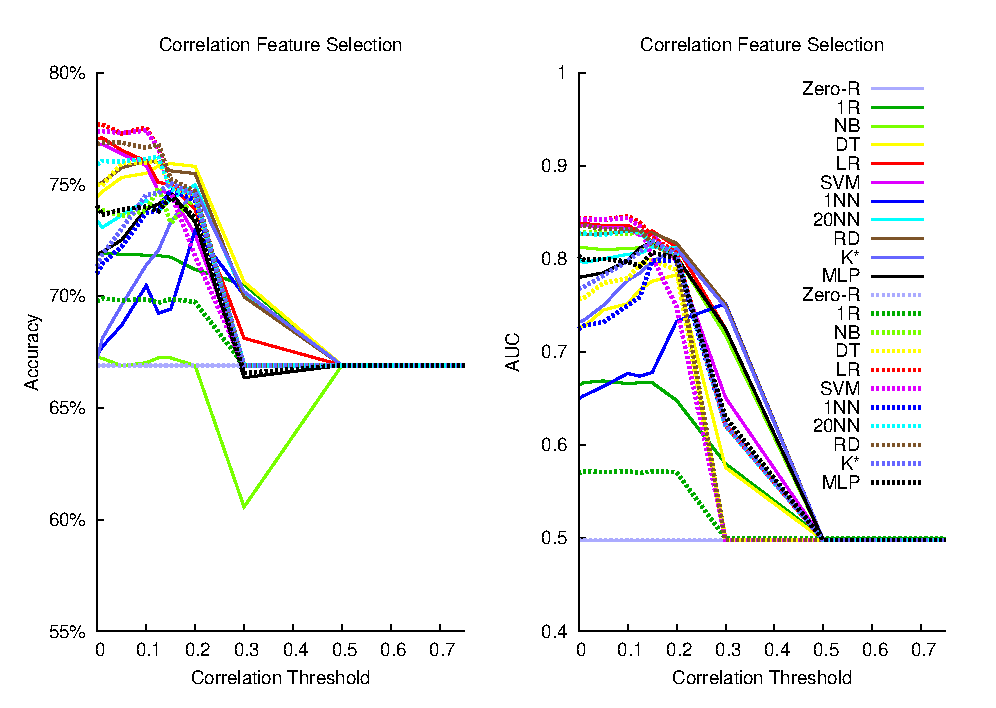
\includegraphics[width=\textwidth]{images/results/tr-corr.eps}
\caption{}
\label{}
\end{subfigure}
\caption{}
\label{}
\end{figure}

\begin{figure}[htbp]
\ContinuedFloat
\begin{subfigure}{\textwidth}
\includegraphics[width=\textwidth]{images/results/tr-ig.eps}
\caption{}
\label{}
\end{subfigure}
\end{figure}

\begin{figure}[htbp]
\ContinuedFloat
\begin{subfigure}{\textwidth}
\includegraphics[width=\textwidth]{images/results/tr-oner.eps}
\caption{}
\label{}
\end{subfigure}
\end{figure}

\subsection{Trauma Data Set}

\subsection{General Data Set}

\section{Effect of Discretisation}

\section{Summary}
